\section{Memory Management}
\label{sec:Managing-Memory}

Let a program $ P \equiv (i_n)_{n \in \mathbb{N}} $ be an ordered sequence of instructions.
Let $ A \subset P $ denote the set of allocation instructions and $ B \subset P $ the deallocation instructions.

\begin{definition}{Memory-safe Program}{memory-safe}
	A program $P$ is \emph{memory-safe} if for all execution paths $\pi \in \Pi(P)$:
	\begin{enumerate}
		\item Exists bijection $T_\pi: A_\pi \rightarrow B_\pi$ where:
		      \begin{itemize}
			      \item $\forall a_i \in A_\pi,\ T_\pi(a_i) = b_i$ is unique.
			      \item $a_i$ lexically precedes $b_i$ on $\pi$.
		      \end{itemize}
		\item The deallocation graph $G_\pi = (V_\pi, E_\pi)$ is acyclic.
		\item $\text{mem}(a_i) \cap \text{mem}(a_j) = \emptyset$ for $i \neq j$.
	\end{enumerate}
\end{definition}

\subsection{Scope-Centralized Memory Management}
\label{subsec:Scope-Centralized-Memory-Management}

\begin{definition}{Memory Arena}{memory-arena}
	A \emph{memory arena} $\mathcal{A} \equiv (\mathcal{M}, F, \Lambda)$ where:
	\begin{itemize}
		\item $\mathcal{M} = \{\mathcal{M}_1,...,\mathcal{M}_k\}$ - is a finite set of disjoint memory blocks..
		\item $F \subseteq \bigcup_{i=1}^k \mathcal{M}_i$ - is the set of free addresses.
		\item $\Lambda$ - is an allocator with allocation strategy $\sigma$.
	\end{itemize}

	The \emph{allocation function} $H: \mathcal{A} \rightharpoonup \mathcal{A} \times \texttt{addr}(\mathcal{M})$ is:
	\[
		H((\mathcal{M}, F, \Lambda)) = \begin{cases}
			((\mathcal{M}, F \setminus \{a\}, \Lambda), a) & \text{if } a \in F \text{ via } \sigma \\
			\text{undefined}                               & \text{otherwise}
		\end{cases}
	\]
	Subject to invariants:
	\begin{enumerate}
		\item Disjointness: $\mathcal{M}_i \cap \mathcal{M}_j = \emptyset\ \forall i \neq j$.
		\item No individual deallocations: $\nexists b_i \in B$ for $a_i \in \mathcal{A}$.
		\item Mass reclamation: $\bigcup \mathcal{M}_\pi \subseteq F_\pi^{\text{final}}$ at scope exit.
	\end{enumerate}
\end{definition}

For control-flow graph $G$ with scope entry/exit nodes $G_a,G_b$:
\begin{itemize}
	\item Arena instantiation at $G_a$ creates $\mathcal{A} = (\mathcal{M}, F, \Lambda)$.
	\item All paths $S_{a\rightarrow b}$ allocate via $H((\mathcal{M}, F, \Lambda))$.
	\item Destruction at $G_b$ enforces $F^{\text{final}} = \bigcup \mathcal{M}$, satisfying Definition~\ref{def:memory-safe}.
\end{itemize}

This formalism reduces verification complexity from $O(2^{|C|})$ paths to $O(1)$ scope-level invariants. The allocator $\Lambda$ implements $\sigma$ through $H$ while maintaining:

\begin{align*}
	\forall \pi \in \Pi(P),\  & \text{1. } T_\pi \text{ bijection} \Rightarrow F^{\text{final}} = \bigcup \mathcal{M} \\
	                          & \text{2. Lexical precedence} \Rightarrow \text{Scope nesting}                         \\
	                          & \text{3. Disjointness} \Rightarrow \mathcal{M}_i \cap \mathcal{M}_j = \emptyset
\end{align*}

\begin{figure}[h]
	\begin{center}
		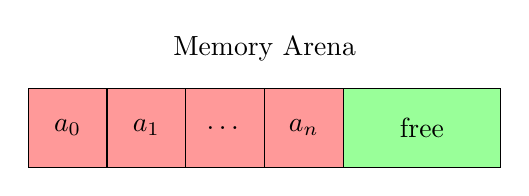
\begin{tikzpicture}
			\draw (0,0) rectangle (6,1);
			\foreach \x in {1,2} {
					\draw (\x,0) -- (\x,1);
				}
			\foreach \x in {2,3,4,5} {
					\shade[left color=green!40!white, right color=green!40!white, draw=black] (2, 0) rectangle (6, 1);
					\draw (5,0.5) node {free};
				}
			\foreach \x/\y in {0/{$a_0$},1/$a_1$,2/\dots,3/$a_n$} {
			\filldraw[fill=red!40!white, draw=black] (\x, 0) rectangle (\x + 1, 1);
			\draw (\x + 0.5, 0.5) node {\y};
			}
			\draw (3,1.5) node {Memory Arena};
		\end{tikzpicture}
	\end{center}
	\caption{Memory arena structure showing sequential allocations within contiguous blocks.}
	\label{fig:memory-arena-illustration}
\end{figure}


\subsection{Initialization-Centralized Memory Management}
\label{subsec:Initialization-Centralized}
We now present a further centralization of memory management through what we shall term the "Defer Pattern," which couples allocation and deallocation at the point of initialization.

Utilizing compiler facilities such as the cleanup attribute in GCC, one may specify:

\begin{verbatim}
MemoryArena *arena DEFER(memory_arena_destroy) = memory_arena_create(...);
\end{verbatim}

This construction guarantees deallocation at scope exit, irrespective of the control flow path that leads to said exit.

The Defer Pattern exhibits the following properties:

\begin{enumerate}
	\item \textbf{Spatial Coupling}: The allocation and its corresponding deallocation are textually adjacent in the source code, providing immediate verification of the appropriate $T_{\pi}(a_i) = b_i$ relationship.

	\item \textbf{Compiler-Enforced Temporal Sequencing}: The compiler ensures that deallocation occurs at scope exit, enforcing the lexical ordering requirement that $a_i$ precedes $b_i$.

	\item \textbf{Single-Point Specification}: Memory management decisions are made once, at the point of initialization, rather than distributed throughout the control flow graph.
\end{enumerate}

\indent
\begin{raggedright}
	This approach effectively centralizes memory management responsibilities at initialization points, delegating enforcement to the compiler. The programmer need only ensure proper declaration of cleanup behaviors at allocation sites, substantially reducing the cognitive burden of tracking allocation-deallocation pairs across the program's control flow structure.
\end{raggedright}

We thus observe a progression from decentralized path-based verification, to scope-centralized arena management, to initialization-centralized specification—each stage reducing the cognitive distance between allocation and deallocation logic, and consequently reducing the opportunity for memory management errors.

For compiler-enforced cleanup:
\[
	\underset{\text{Allocation}}{\underbrace{\text{MemoryArena}^* \mathcal{A}}}
	\ \underset{\text{Deallocation}}{\xrightarrow{\text{DEFER}}}
	\underset{\text{Scope exit}}{\mathcal{A} \mapsto (\mathcal{M}, F^{\text{final}}, \Lambda)}
\]

where the DEFER macro enforces:
\[
	\mathcal{A} \mapsto (\emptyset, \bigcup \mathcal{M}, \Lambda)\ \forall \pi \in \Pi(P).
\]
\newpage
